\chapter{To verify truth table for OR gate}
%\ref{sec:background}.

%\section{Aim}
%\label{sec:objectives}
%	To verify the truth table for AND Gate.

\section{Apparatus}
%\label{sec:objectives}
	\begin{itemize}
		\tightlist
		\item Kit for realization of gates
		\item Connecting Leads
	\end{itemize}

\section{Theory}
	The OR gate is an electronic circuit that gives a high output (1) if one or more of its inputs are high. A plus (+) is used to show the OR operation.
	\begin{figure}[h]
		\centering
		
\includegraphics{img/exp2/1}
		\caption{Symbol for OR gate}
		\label{fig:2:1}
	\end{figure}
	\begin{figure}[h]
		\centering
		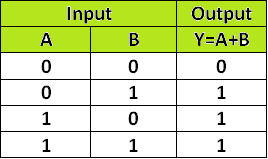
\includegraphics{img/exp2/2}
		\caption{Truth Table for OR gate}
		\label{fig:2:2}
	\end{figure}
	OR gate can be realized by DRL (Diode-Resistance-Logic) or by TTL (Transistor-Transistor-Logic). Presently, we will learn how to implement the OR gate using DRL (Diode-Resistance-Logic). To realise OR gate, we will use a diode at every input of the OR gate. The anode part of diode is connected with input while the cathode part is joined together and a resistor, connected with the cathode is grounded. In this case, we have taken two inputs which can be seen in the circuit below.
	
	When both the inputs are at logic 0 or low state then the diodes D1 and D2 become reverse biased. Since the anode terminal of diode is at lower voltage level than the cathode terminal, so diode will act as open circuit so there is no voltage across resistor and hence output voltage is same as ground. When either of the diodes is at logic 1 or high state then the diode corresponding to that input is forward bias. Since this time anode is at high voltage than cathode therefore current will flow through forward biased diode and this current then appears on resistor causing high voltage at output terminal also. Hence at output we get high or logic 1 or +5V. So, if any or both inputs are high, the output will be high or “1”.
	
	\begin{figure}[h]
		\centering
		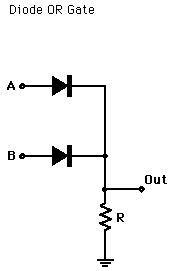
\includegraphics[width=0.3\linewidth]{img/exp2/3}
		\caption{Circut for making OR gate}
		\label{fig:2:3}
	\end{figure}
				
\section{Procedure}
	\subsubsection{Simulator 1}
	\begin{itemize}
		\tightlist
		\item Connect the supply(+5V) to the circuit.
		\item Press the switches for inputs "A" and "B".
		\item The bulb glows if any one or both the switches are ON else it won't glow.
		\item Repeat step-2 and step-3 for all state of inputs.
	\end{itemize}

	\subsubsection{Simulator 2}
	\begin{itemize}
		\tightlist
		\item Enter the Boolean input "A" and "B".
		\item Enter the Boolean output for your corresponding inputs.
		\item Click on "Check" Button to verify your output.
		\item Click "Print" if you want to get print out of Truth Table.
	\end{itemize}


\section{Observations}
	\begin{figure}[h]
		\centering
		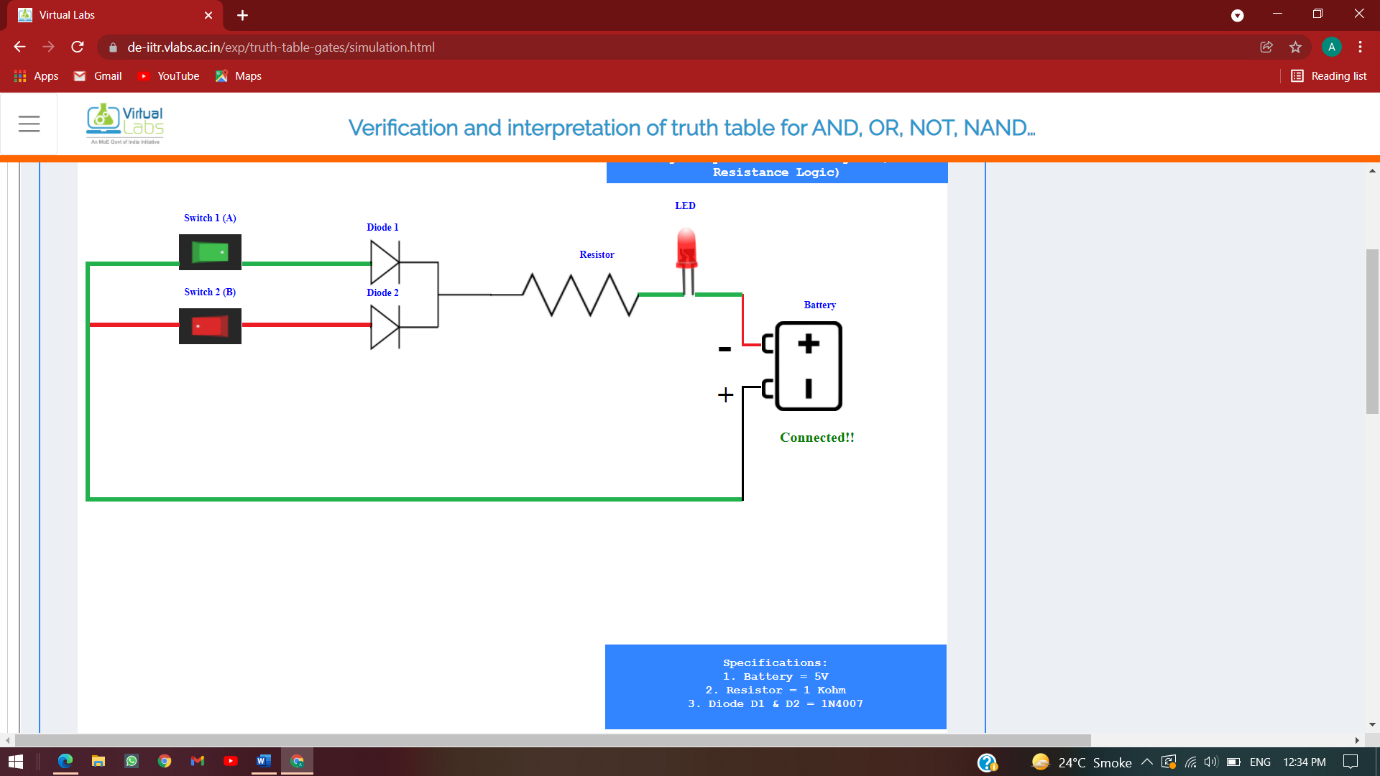
\includegraphics[width=0.9\linewidth]{img/exp2/4}
		\caption{}
		\label{fig:2:4}
	\end{figure}
		\begin{figure}[h]
		\centering
		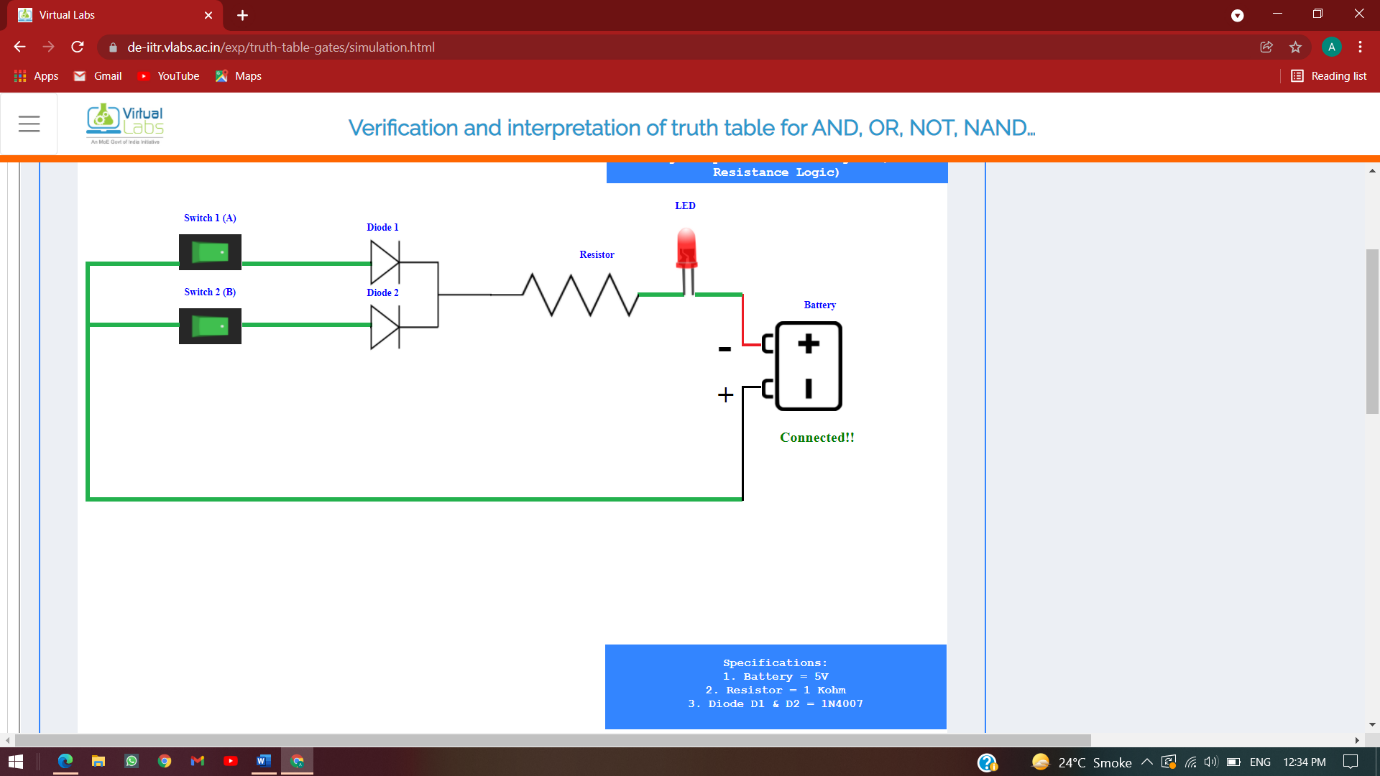
\includegraphics[width=0.9\linewidth]{img/exp2/5}
		\caption{}
		\label{fig:2:5}
	\end{figure}
		\begin{figure}[h]
		\centering
		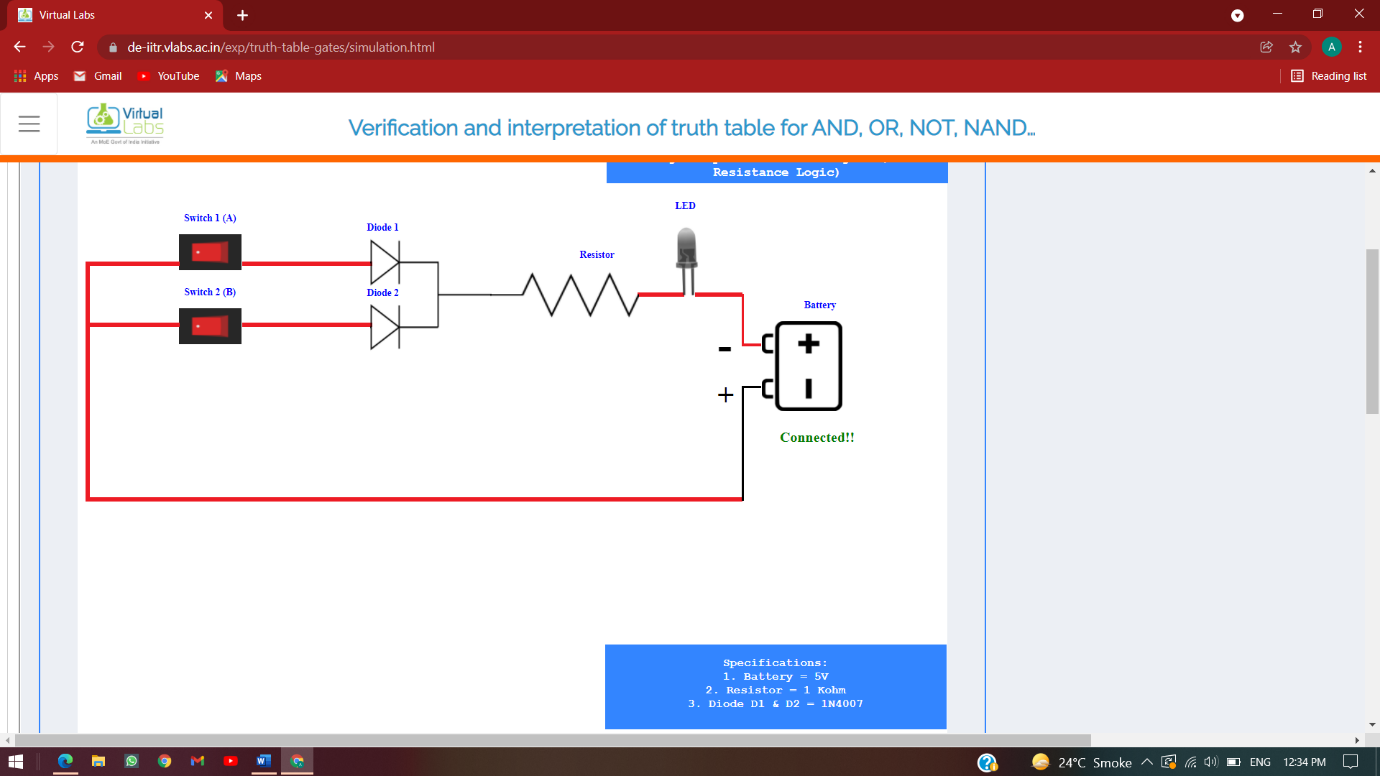
\includegraphics[width=0.9\linewidth]{img/exp2/6}
		\caption{}
		\label{fig:2:6}
	\end{figure}
		\begin{figure}[h]
		\centering
		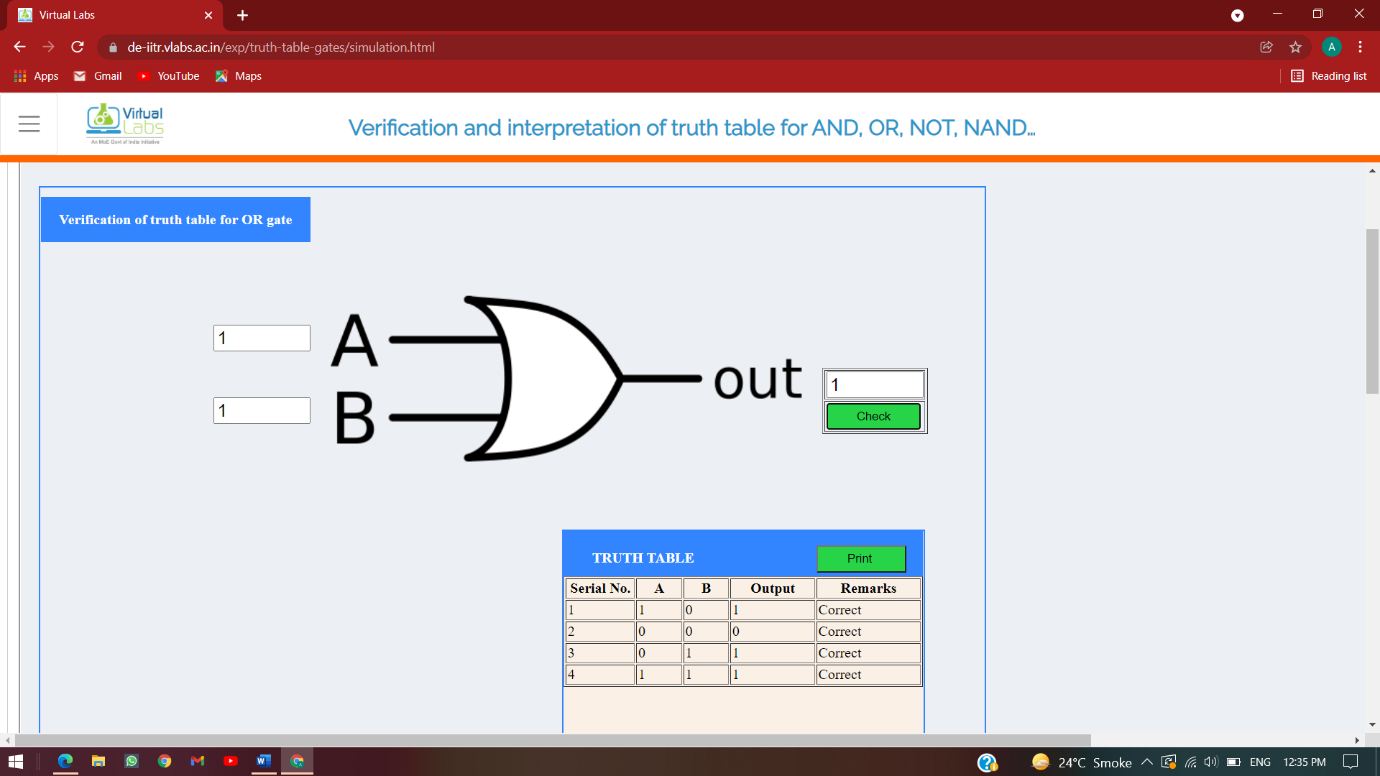
\includegraphics[width=0.9\linewidth]{img/exp2/7}
		\caption{}
		\label{fig:2:7}
	\end{figure}

\section{Conclusion}
Thus we can see that when both inputs are low then only the output is low otherwise it is high when even one of the inputs is high.

\section{Precautions}
	\begin{enumerate}
		\tightlist
		\item Make the connections when power supply is OFF.
		\item Ensure that the connections are tight.
		\item Change the status of inputs only when power supply is OFF.
	\end{enumerate}